\chapter{Proposed Solution : Deep Stream System}
\section{Overall Pipeline Structure}
The deployed system implements a multi-stage, distributed intelligent video analytics pipeline designed for real-time people counting. The architecture begins on a Windows host machine, where an input image is first processed by a Super Resolution (SR) deep learning model to enhance its visual quality. The output of this SR model, an improved-quality image, is then assemble to a video, encoded and transmitted over the local network via the Real-Time Streaming Protocol (RTSP). An NVIDIA Jetson device, acting as the primary analytics engine, subscribes to this RTSP stream. On the Jetson, the DeepStream SDK is utilized to construct a GStreamer pipeline that ingests the enhanced video, performs hardware-accelerated decoding, and feeds the frames into a custom-trained people counting model for inference. The resulting people count is then visualized as an on-screen display overlaid on the video, which is rendered on a connected monitor. This distributed approach leverages the Windows machine for initial image enhancement and the specialized capabilities of the Jetson and DeepStream for efficient, real-time AI inference and analytics.
\begin{figure}[H]
    \centering
    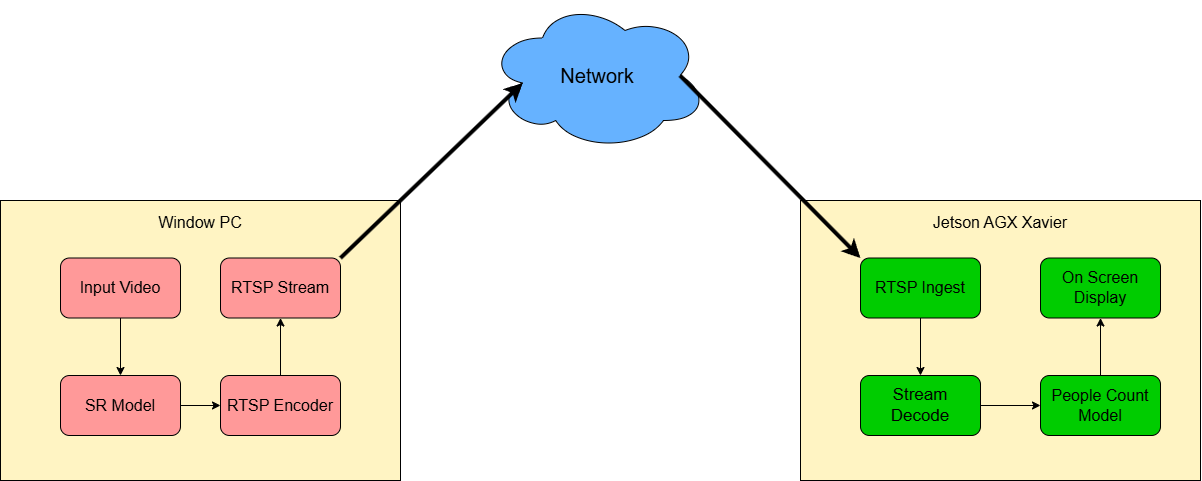
\includegraphics[width=1\linewidth]{related-work/image/Overall_pipeline.png}
    \caption{System Overall Pipeline}
    \label{fig:enter-label}
\end{figure}

\section{Window Host}
The initial stage of our proposed solution, executed on a Windows PC, is dedicated to transforming a sequence of input images into a high-quality, streamable RTSP feed. Each image in the input sequence is first individually processed by a Super Resolution (SR) model. This step enhances the resolution and detail of every image, which is critical for improving the accuracy of the subsequent people counting task. Once the SR processing is complete for each image:
\begin{figure}[H]
    \centering
    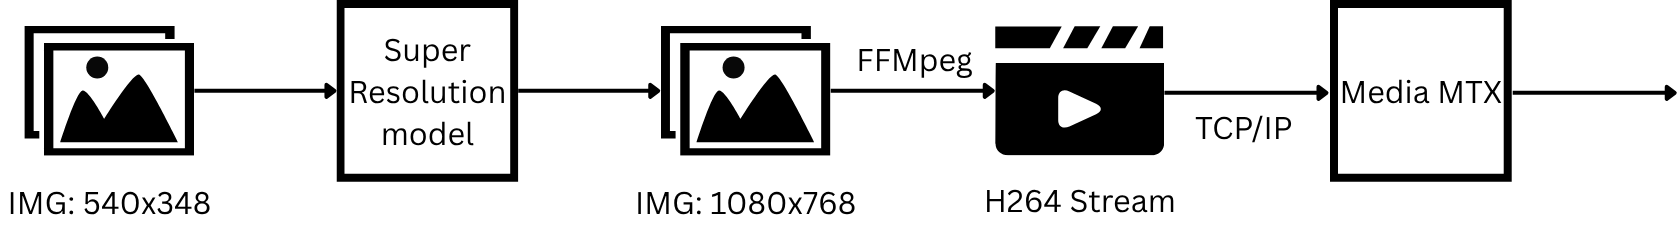
\includegraphics[width=1\linewidth]{related-work/image/window_pipeline.png}
    \caption{Window Pipeline}
    \label{fig:enter-label}
\end{figure}
\begin{itemize}
    \item \textbf{Image Sequence to Video Conversion \& Encoding (FFmpeg):} FFmpeg is invoked with specific parameters to read the sequence of SR-enhanced images. The input presentation rate for these images is controlled by framerate (each image is sourced for 3 seconds). These images are then encoded into an H.264 video stream using the libx264 encoder. To prioritize real-time performance and low latency, the encoding employs -preset ultrafast and -tune zerolatency, with -pix\_fmt yuv420p ensuring broad compatibility for decoding. The output video resolution is explicitly set to the detected image dimensions (-s {width}x{height}), and the final stream's framerate is set by -r (your STREAM\_FPS variable, e.g., 40 fps), which means FFmpeg will duplicate frames if STREAM\_FPS is higher than the effective input image presentation rate.
    \item \textbf{RTSP Stream Publishing (FFmpeg to Mediamtx):} Once encoded, FFmpeg packages the H.264 video into the Real-Time Streaming Protocol (RTSP) format . It then acts as an RTSP client, publishing this stream typically using TCP for reliability to a predefined URL . It is at this URL that Mediamtx is expected to be listening, ready to receive the incoming stream from FFmpeg.
    \item \textbf{Stream Serving (Mediamtx): }Mediamtx, running independently, serves as the dedicated RTSP broker. It ingests the stream published by FFmpeg and manages its distribution, making the enhanced video feed available over the network to subscribing clients, primarily the Jetson device in the subsequent stage of the pipeline.

\end{itemize}

\section{Jetson AGX Xavier}
On the NVIDIA Jetson platform, the DeepStream SDK orchestrates a sophisticated GStreamer pipeline to process the incoming super-resolved RTSP video streams from the Windows host. This pipeline is designed for optimal GPU utilization and real-time performance, handling maximum 4 concurrent streams.
\begin{figure}[H]
    \centering
    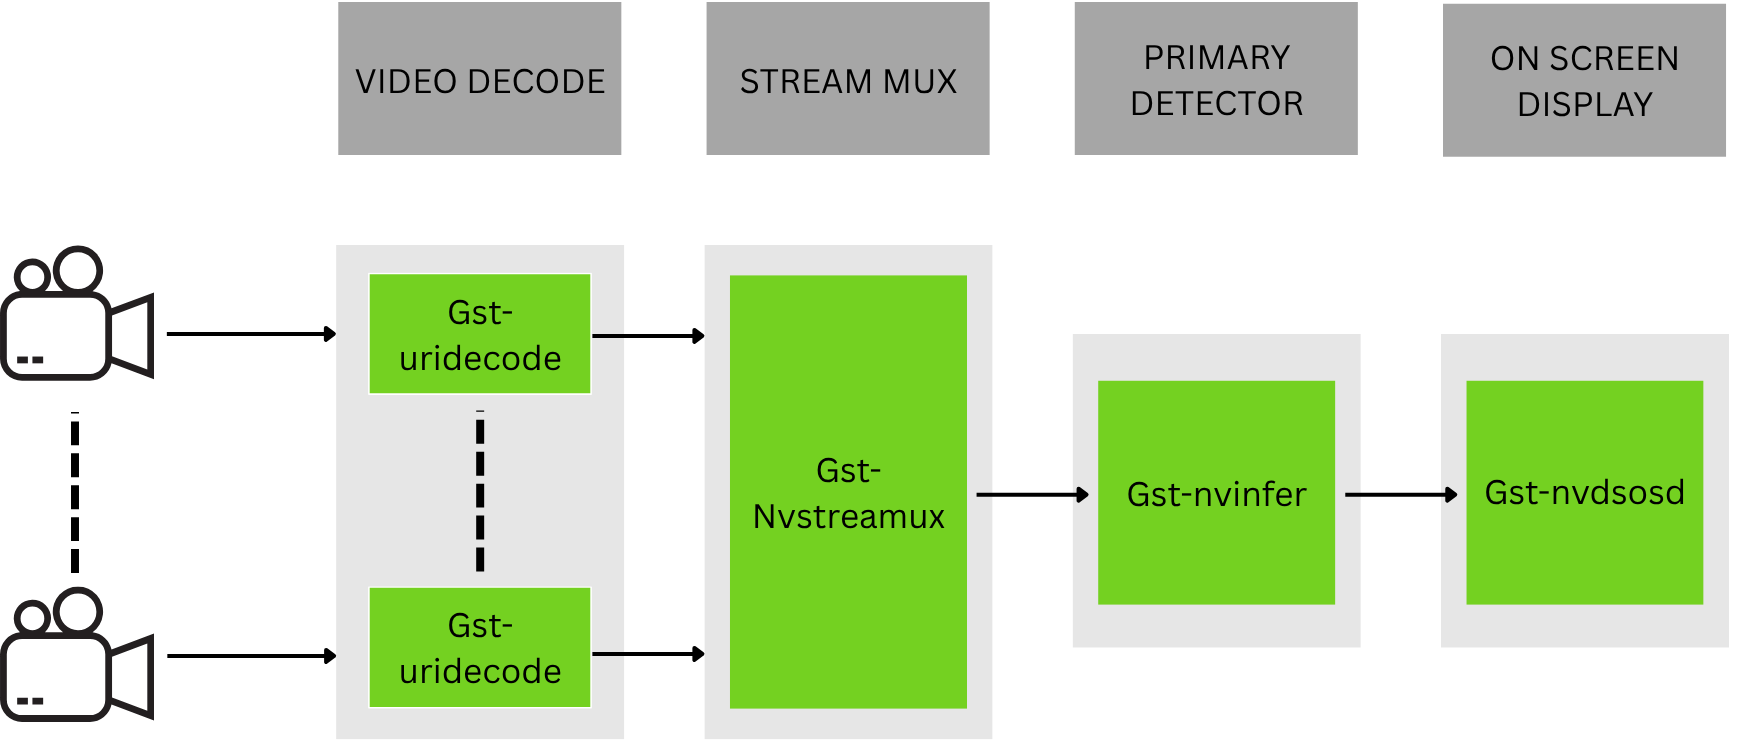
\includegraphics[width=1\linewidth]{related-work/image/pipeline_jetson.png}
    \caption{Deepstream Pipeline}
    \label{fig:enter-label}
\end{figure}
\begin{itemize}
    \item \textbf{Source Input Bin} (\verb|uridecodebin|):
        \begin{itemize}
            \item \textbf{Purpose: }To connect to the RTSP stream, receive its data, depayload it, parse the video codec, and decode it into raw video frames.
            \item \textbf{Implementation:} Using \verb|uridecodebin| for multiple sources in the pipeline and accepting any type of input (e.g. RTSP/File), any GStreamer supported container format, and any codec.
            \item \textbf{Output:} A stream of video/x-raw(memory:NVMM) frames from the RTSP source.
        \end{itemize}
    \item \textbf{Stream Multiplexer} (\verb|nvstreammux|):
        \begin{itemize}
            \item \textbf{Purpose: }\verb|nvstreammux| is essential in DeepStream pipelines. It prepares the stream for \verb|nvinfer| by creating batches, handling buffer allocation, and scaling the video.
            \item \textbf{Input: }Receives the single video/x-raw(memory:NVMM) stream on its sink pad from the source bin
            \item \textbf{Output: }A GStreamer buffer containing a batch of maximum 4 frame (512x512) in video/x-raw(memory:NVMM) format
        \end{itemize}
    \item \textbf{Primary GIE - People Counting} (\verb|nvinfer|):
        \begin{itemize}
            \item \textbf{Purpose: }Executes the custom TensorRT people counting model on the frames received from \verb|nvstreammux|.
            \item \textbf{Output: }Passes through the video frame, along with the calculation result. The probe then finds the "number\_of\_people" output layer, extracts the count, and prepares for \verb|nvdsosd|.
        \end{itemize}
    \item \textbf{On-Screen Display} (\verb|nvdsosd|):
        \begin{itemize}
            \item \textbf{Purpose: }Display the video, along with the text "People Count" and calculating FPS when the application terminates.
        \end{itemize}
\end{itemize}